\chapter{Θέματα 2, 3, 4}
Στα θέματα 2, 3, 4 κληθήκαμε να εφαρμόσουμε την μέθοδο Μέγιστης Καθόδου που υλοποιήσαμε για να βρούμε το ελάχιστο της γνωστής συνάρτησης $f$. Το παραπάνω έπρεπε να γίνει με ακρίβεια $\epsilon = 0.01$ για κάθε μία από τις παρακάτω περιπτώσεις $\gamma$:
\begin{enumerate}
    \item $\gamma_k = 0.5, s_k = 5, x_0 = (5, -5)$
    \item $\gamma_k = 0.1, s_k = 15, x_0 = (-5, 10)$
    \item $\gamma_k = 0.2, s_k = 0.1, x_0 = (8, -10)$
\end{enumerate}

Για την περίπτωση 1:\newline
Η μέθοδος δεν συνέκλινε. Αντιθέτως το σημείο άρχισε να ταλαντώνεται γύρω από το σημείο ελαχίστου επ' αόριστον και η μέθοδος τερμάτισε μόνο όταν έφτασε τον μέγιστο αριθμό επαναλήψεων που είχε οριστεί ως δικλίδα ασφαλείας. Το αποτέλεσμα είναι λογικό, καθώς η ανάλυση του \cref{sec:convergence} για το $\gamma$ ισχύει και στην παρούσα περίπτωση, ωστόσο για το $\gamma' = \gamma_k \cdot s_k$, το οποίο στην περίπτωση μας ισούται με $2.5$.
\begin{figure}[!h]
    \centering
    \subfloat[Convergence in 1D space]{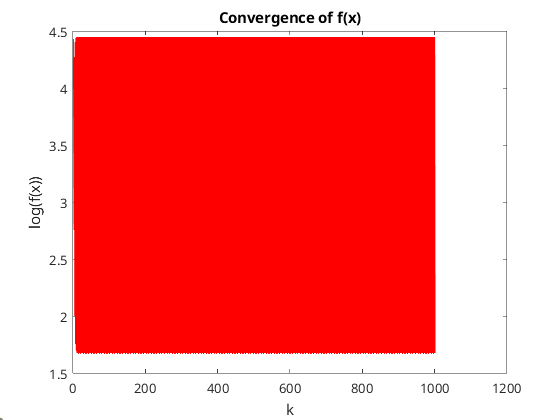
\includegraphics[width=0.5\textwidth]{Figs/conv_2.png}}
    \hfill
    \subfloat[Convergence in 2D space]{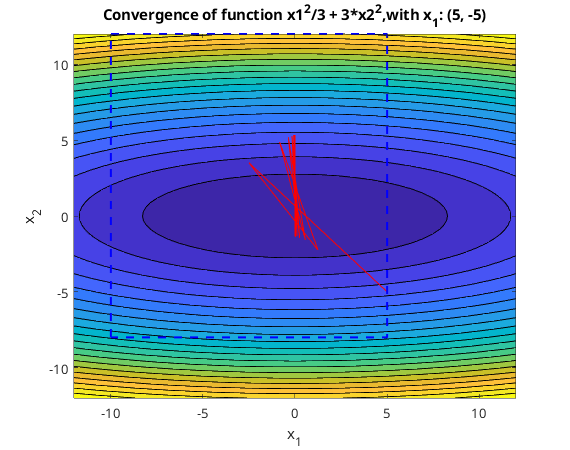
\includegraphics[width=0.5\textwidth]{Figs/2.png}}
\end{figure}
\sep
Για την περίπτωση 2:\newline
H μέθοδος συνέκλινε και βρήκε ελάχιστο το $0$ στο σημείο $x^* = (0, 0)$, έπειτα από 200 επαναλήψεις. Η μέθοδος ενδεχομένως συνέκλινε από τύχη (κάτι που παρατηρείται και στο μονοδιάστατο διάγραμμα σύγκλισης που δεν είναι ομαλό), καθώς θεωρητικά το $\gamma_k \cdot s_k = 1.5$, δηλαδή πάνω από 0.33. Ένας απλός τρόπος να σιγουρέψουμε την σύγκλιση θα ήταν η μείωση του $s_k$ πχ. $s_k = 3$.
\begin{figure}[H]
    \centering
    \subfloat[Convergence in 1D space]{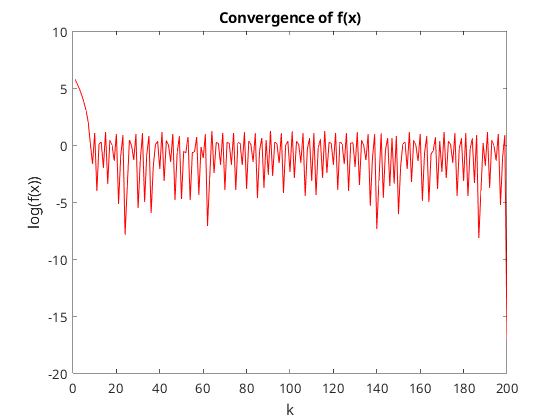
\includegraphics[width=0.5\textwidth]{Figs/3_conv.png}}
    \hfill
    \subfloat[Convergence in 2D space]{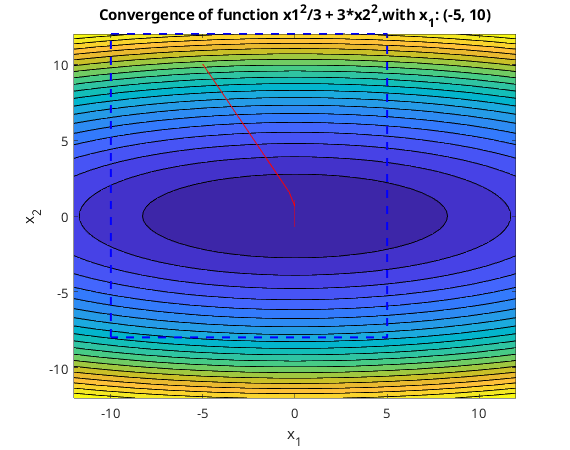
\includegraphics[width=0.5\textwidth]{Figs/3.png}}
\end{figure}
Για την περίπτωση 3:\newline
Παρατηρούμε ότι το αρχικό σημείο βρίσκεται εκτός περιορισμών. Θα εφαρμόσουμε τη μέθοδο επομένως με αρχικό σημείο την προβολή του, δηλαδή το $x_0 = (5, -8)$. (Παρόλο που λόγω περιέργειας η μέθοδος δοκιμάστηκε και στο αρχικό σημείο και συγκλίνει κανονικά). H μέθοδος συνέκλινε και βρήκε ελάχιστο το $0$ στο σημείο $x^* = (0.015, 0)$, έπειτα από 434 επαναλήψεις. Η σύγκλιση στο ελάχιστο γίνεται πολύ πιο αργά και ομαλά σε σχέση με την προηγούμενη περίπτωση, καθώς το $s_k$ είναι 150 φορές μικρότερο, ενώ το $\gamma$ μόλις δύο φορές μεγαλύτερο. Βλέπουμε λοιπόν πως η ταχύτητα σύγκλισης εξαρτάται και από την επιλογή της παραμέτρου $s$, πέραν του $\gamma$.
\begin{figure}[!h]
    \centering
    \subfloat[Convergence in 1D space]{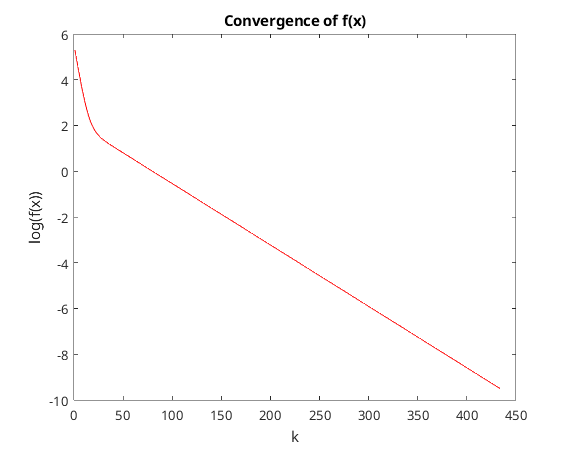
\includegraphics[width=0.5\textwidth]{Figs/4_conv.png}}
    \hfill
    \subfloat[Convergence in 2D space]{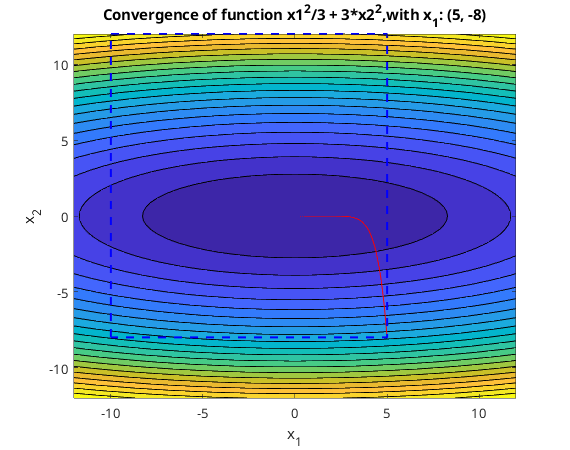
\includegraphics[width=0.5\textwidth]{Figs/4.png}}
\end{figure}